\documentclass[12pt, a4paper]{article}
\usepackage{graphicx}
\usepackage{array}
\usepackage[T2A]{fontenc}
\usepackage[utf8]{inputenc}
\usepackage[english,russian]{babel}
\usepackage{color}

% PDF Search & cut'n'paste
\usepackage{cmap}

% Indent the first paragraph as well
\usepackage{indentfirst}

% According to GOST, sections should be called chapters in diploma
\usepackage{titlesec}

% Detect whether PDFLaTeX is in use
\usepackage{ifpdf}

% Graphics
\ifpdf
    \usepackage[pdftex]{graphicx}
\else
    \usepackage{graphicx}
\fi

% Hyperlinks
\ifpdf
        \usepackage[pdftex]{hyperref}
\else
        \usepackage{hyperref}
\fi

\hypersetup{
        unicode=true,
        pdftitle={
        },
        pdfauthor={},
        pdfkeywords={
        },
        colorlinks,
        citecolor=black,
        filecolor=black,
        linkcolor=black,
        urlcolor=blue
}

% Russian-styled figure and table captions
\usepackage[labelsep=period]{caption}
% This declaration makes TeX less fussy about line breaking. This can
% prevent overfull boxes, but may leave too much space between words.
% As this really isn't a fine art typography, we'll turn it on, so
% we won't have paragraphs which spans on the margins...
\sloppy

% Page numbering at the right topmost part of the page
\pagestyle{myheadings}

\usepackage{listings}
\let\stdsection\section
\renewcommand\section{\newpage\stdsection}
\definecolor{lightgray}{rgb}{.9,.9,.9}
\definecolor{darkgray}{rgb}{.4,.4,.4}
\definecolor{purple}{rgb}{0.65, 0.12, 0.82}
\graphicspath{{./images/}}
\lstdefinelanguage{JavaScript}{
  keywords={typeof, new, true, false, catch, function, return, null, catch, switch, var, if, in, while, do, else, case, break},
  keywordstyle=\color{blue}\bfseries,
  ndkeywords={class, export, boolean, throw, implements, import, this},
  ndkeywordstyle=\color{darkgray}\bfseries,
  identifierstyle=\color{black},
  sensitive=false,
  comment=[l]{//},
  morecomment=[s]{/*}{*/},
  commentstyle=\color{purple}\ttfamily,
  stringstyle=\color{red}\ttfamily,
  morestring=[b]',
  morestring=[b]"
}
\lstset{
   language=JavaScript,
   backgroundcolor=\color{lightgray},
   extendedchars=true,
   basicstyle=\footnotesize\ttfamily,
   showstringspaces=false,
   showspaces=false,
   numbers=left,
   numberstyle=\footnotesize,
   numbersep=9pt,
   tabsize=2,
   breaklines=true,
   showtabs=false,
   captionpos=b
}
\linespread{1.5}
%% TODO Нормальная титульная страница
\author{Андрей Лушников}
\title{Разработка и реализация алгоритмов деформирования трехмерной геометрии
анатомии человека на основе WebGL}
\date{Апрель 2012 год}

\begin{document}
\maketitle

\tableofcontents
\newpage

\section{Постановка задачи}
Каждый программный продукт на протяжении всех стадий жизни сопровождает много
разнообразных проблем. Это и проблемы его поддержки, и проблемы переносимости, и
проблемы контроля версий и устаревания. Эти проблемы характерны как для рядовых
программ, которые знакомы каждому пользователю, так и для специализированных
программ, используемых врачами в их ежедневной практике для оценки,
визуализирования и прогнозирования результатов пластических операций. Один из
современных подходов к распространению программного обеспечения, носящий
название ``Software as a Service'' - призван решить целый класс таких проблем.

Software-as-a-Service (далее ``SAAS'') - модель использования программного
обеспечения, при которой программный продукт выполнен в виде Web-приложения, и
разработчик самостоятельно управляет его развитием. Пользователи имеют доступ к
приложению через сеть интернет, при этом они избавлены от затрат, связанных с
установкой, обновлением и поддержкой работоспособности оборудования и
работающего на нем программного обеспечения.

Программное обеспечение, разработанное специально для врачей и решающее
различные медицинские задачи, зачастую также обладает большим количеством
недостатков.  Оно не кросс платформенное, а его установка зачастую трудоемка.
Оно предъявляет дополнительные требования к рабочим станциям врачей, что сужает
область применения.

Основной задачей данной дипломной работы было разработать программный редактор,
позволяющий загружать и обозревать трехмерную модель, а так же алгоритм,
позволяющий пользователю изменять части геометрии загруженной модели.
Разработанное приложение должно полностью следовать модели SAAS, что избавило бы
его от большого количества недостатков, присущих программному обеспечению в
общем и медицинскому программному обеспечению в частности. Программный редактор
должен был быть как можно менее зависим от конфигурации клиентской платформы, что
упростило бы его использование в больницах. Отдельным достоинством приложения
была бы возможность использования на планшетных компьютерах.

В новом редакторе необходимо было дополнительно исследовать и поддержать
возможность переиспользования программных модулей, написанных на С++ для ранее
разработанных desktop-приложений.  Реализация такой возможности позволяет не
только переиспользовать унаследованный от предыдущих проектов код, но и дает
возможность описывать и выполнять сложные вычисления на компилируемых и
хорошо-оптимизируемых языках программирования, что выливается в прирост
производительности.

\section{Архитектура}

\subsection{Описание архитектуры}

Для выполнения поставленных целей было решено использовать клиент-серверную
архитектуру. В роли клиента выступает web-приложение, предоставляющее
пользователю необходимый интерфейс для взаимодействия, а серверная часть
отвечает за конвертацию OBJ-файлов и выполнение серверных вычислений. Обе части
взаимодействуют между собой по средствам технологии AJAX и специально
разработанного для целей приложения протокола, основанного на сообщениях в
формате JSON особого вида. Таким образом взаимодействие между компонентами системы
происходит по средствам внешнего API, предоставленного серверной частью,
что соответствует принципу инкапсуляции и способствует заменяемости
любого из компонентов архитектуры.

\subsubsection{Клиент}

Клиентская часть была реализована в виде web-приложения, написанного
на HTML5.0 и Javascript. Для отображения графики используется
перспективная технология WebGL.

WebGL - это библиотека для программного обеспечения, которая расширяет
возможности языка программирования JavaScript, позволяя ему создавать
интерактивную 3D графику внутри любого совместимого с ней web-браузера. Код на
WebGL выполняется с помощью вычислительных ресурсов видеокарты. Технология
разрабатывается промышленным консорциумом Khronos Group, который
специализируется на выработке открытых стандартов интерфейсов программирования в
области создания и воспроизведения динамической графики и звука. Активное
участие в разработке и внедрении стандарта так же принимают разработчики
браузеров Apple Safari, Google Chrome, Mozilla Firefox, Opera,  а также
специалисты компаний AMD и NVidia. На данный момент технология поддерживается в
последних версиях браузеров Safari, Mozilla, Opera и Chrome, а так же в браузере
Internet Explorer при использовании специального дополнения IEWebGL. Среди
мобильных устройств данная технология уже поддерживается в браузере телефона
Nokia N900, а так же в Safari Mobile начиная с версии операционной системы iOS
4.2.

Выбор технологии WebGL в качестве средства для отображения трехмерной графики
преследует цель достижения кросс-платформенной реализации. Перспективы развития
этой технологии в отношении рынка мобильных платформ являются самыми
многообещающими по сравнению с остальными кросс-платформенными технологиями.
\footnote{стоит отметить, что использование WebGL разрешено в браузере Mobile
Safari только в контексте рекламных объявлений iAd}

\subsubsection{Сервер}

Cервеная часть была реализована с использованием технологии с открытым исходным
кодом``Node.js''. Эта технология позволяет исполнять JavaScript на стороне
сервера, причем в качестве виртуальной машины для исполнения JavaScript-кода
используется высокопроизводительная V8, разработанная компанией Google и
используемая в браузере Google Chrome.

``Node.js'' - платформа с открытым исходным кодом для построения приложений,
основанных на асинхронных I/O операциях с использованием языка JavaScript.
Несмотря на распространенное мнение, платформа не является первой в своем роде и
в некотором роде наследует принципы, заложенные в асинхронном I/O фреймворке
``EventMachine'' для языка программирования Ruby. Однако большим достоинством
этой платформы перед ``EventMachine'' можно назвать язык программирования
EcmaScript стандарта 5.0, или JavaScript, применяемый на платформе ``Node.js'' и
исторически ориентированный на асинхронные взаимодействия.  Благодаря отсутствию
в его спецификации I/O операций (что в некотором смысле удивительно для
web-ориентированного языка), появилась возможность создать необходимую
библиотеку асинхронных I/O операций, которая и стала стандартной при
использовании ``Node.js''-приложений.

Использование одного и того же языка на стороне клиента и сервера дает несколько
достоинств разработчикам. В первую очередь появляется возможность эффективного
переиспользования одного и того же кода как на клиентской, так и на серверной
частях приложения. Примером такого переиспользования может служить
код проверки данных формы, который из соображений безопасности и целостности
обязан присутствовать на стороне сервера, а из соображений удобства пользования
интерфейсом и минимизации клиент-серверных взаимодействий должен быть также и на
клиентской стороне.

Интересной особенностью технологии ``Node.js'', используемой в качестве серверной
платформы, можно назвать высокую производительность и чрезвычайно легкую
масштабируемость. Эти особенности связаны с асинхронной моделью чтения и записи
данных. Таким образом, в противоположность классическому web-серверу,
запускающему обработку каждого запроса в отдельном потоке, но выполняющем в этом
потоке синхронные операции, ``Node.js'' использует только один системный поток.
В случае необходимости масштабирования ``Node.js'' серверов, можно запустить
несколько серверов приложения, объединив их по средством обратного proxy с
балансером. Таким образом приложение, разработанное на этой платформе,
фактически не имеет потолка по обрабатываемой нагрузке.

За время своего существования серверная платформа ``Node.js'' обросла большой
инфраструктурой. Благодаря наличию фреймворка Connect, ставшего стандартом
де-факто для приложений и задавшего стандарт для разработки сторонних модулей,
разработчикам доступно большое количество модулей. Менеджер пакетов обеспечивает
централизованный доступ и быструю установку сторонних модулей, становится
возможным быстрое прототипирование как самого приложения, так и его отдельных
возможностей.

Несмотря на то, что преимущества от использования динамического
слабо-типизированного прототипно-ориентированного языка на стороне сервера
заметны далеко не сразу, ввиду выше указанных причин является
обоснованным и оправданным.

\subsubsection{Переиспользование унаследованного кода}

Для поддержания возможности переиспользования модулей и алгоритмов, написанных
на языке программирования С++ для ранее разработанных desktop-приложений,
используется технология Apache Thrift.

Эта технология была разработана в Facebook по аналогии с Google Protocol Buffers
и служит для написания приложений на нескольких языках программирования. Thrift
представляет собой транскомпилятор, преобразующий файл описания данных и
сигнатуры методов, предназначенных для удаленного вызова, на любой из
поддерживаемых языков\footnote{Thrift версии 0.8.0 поддерживает 20 языков}.

С помощью этой технологии серверная часть приложения получила возможность
вызывать методы, написанные на языках программирования, отличных от JavaScript.
Однако так как вся информация о состоянии геометрии находится на клиенте, то
отдельно было реализовано дополнительное клиент-серверное взаимодействие,
передающее текущую информацию о геометрии с клиента на сервер. Таким образом,
была реализована следующая схема

\begin{enumerate}
    \item Данные о состоянии геометрии на клиенте кодируются в соответствии с
    установленным форматом клиент-серверного взаимодействия и по протоколу HTTP
    передаются на сервер
    \item Сервер получает состояние геометрии и передает ее в качестве аргумента
    при вызове удаленного метода, в нашем случае реализованного на языке C++.
    За вызов удаленного метода отвечает технология Thrift
    \item Результаты работы метода возвращаются на сервер. Полученный ответ
    кодируется в соответствии с форматом клиент-серверного взаимодействия и по
    протоколу HTTP отправляются обратно на клиент.
    \item Клиент, получив ответ, применяет новую геометрию к объекту.
\end{enumerate}


\subsection{Альтернативы}

В процессе выбора технологий для решения поставленных задач было
рассмотрено множество альтернативных решений для каждого из участков
архитектуры. Каждое из таких решений было оценено в соответствии с
поставленной задачей и предъявляемыми к ней требованиями. Результаты
этого исследования определили выбор в пользу описанных технологий. Ниже
приведены решения и подходы, рассмотренные в качестве альтернатив для
реализации поставленных задач, и дан их краткий анализ.

\subsubsection{Flash на стороне пользователя}

При разработке интерактивных web-приложений большую популярность снискала
технология Flash, позволяющая создавать графически богатые интерфейсы. Для
работы этой технологии в браузере необходимо специальное дополнение,
устанавливающееся пользователем отдельно. За счет
своей распространенности технология обладает обширным сообществом, большим
количеством учебных материалов и многочисленными движками для обработки и
отображения трехмерной графики.

Несмотря на вышеперечисленные достоинства, технология Flash на данных момент не
поддерживается ни на одной из популярных мобильных платформ. Компания Adobe,
владеющая всеми правами на технологию Flash и являющаяся единственным ее
разработчиком, официально отказалась от развития мобильного направления развития
платформы. В задачи данной работы входило создание кросс-платформенного
приложения, в том числе способного выполняться на планшетных компьютерах. Ввиду
отсутствия такой теоретической возможности, от этой технологии было решено
отказаться.

\subsubsection{Использование 3D-фреймворка Unity}

Платформа Unity зарекомендовала себя в качестве мощного средства создания
двумерных и трехмерных приложений под консоли и настольные компьютеры под
управлением OS X и Windows. Кроме того, платформа занимает свою нишу в области
web-приложений, предоставляя разработчикам разрабатывать браузерные игры на
Unity и использованием одной из следующих опций

\begin{itemize}
    \item Использование специального дополнения для браузера, исполняющего код
    Unity-приложений. Это дополнение должно быть установлено пользователем.
    \item Использование экспериментального движка на основе Flash. У
    пользователя должно быть установлено дополнение, позволяющее исполнять код
    технологии Flash.
\end{itemize}

К сожалению, ни одна из предложенных опций не поддерживается на мобильных
системах. Однако, благодаря кросс-платформенной сущности движка, существует
возможность перекомпилировать приложения, написанные с использованием этой
технологии, под целевые платформы. Такое решение позволяет покрыть мобильный
сегмент, однако не соответствует модели распространения SAAS, из-за чего от
технологии было решено отказаться.

\subsubsection{Использование Ruby on Rails}

Ввиду поставленных задач возникла необходимость использования серверной части в
архитектуре приложения. При разработке любого серверного решения
акценты ставятся на вопросы масштабирования, а так же возможности быстрого
прототипирования приложения. Используемый фреймворк должен
поддерживать роутинг запросов соответствующим обработчикам и поддерживать
шаблоны для генерации html-страниц. Этим параметрам удовлетворяют
несколько популярных серверных решений: фреймворк ``Ruby on Rails'', фреймворк
``Django'' и платформа ``Node.js'' с серверным фреймворком ``Express.js''. Ввиду
концептуальной схожести фреймворков ``Ruby on Rails'' и ``Django'' ограничимся сравнением Ruby on Rails и ``Node.js''.


``Ruby on Rails'' является более солидным и развитым проектом, нежели
``Express.js''. Обе платформы предлагают менеджеры пакетов и большую библиотеку
общедоступных open-source решений для самых разных задач, что делает
прототипирование одинаково легким на обоих платформах. Однако использование
``Ruby on Rails'' налагает на разработчика необходимость конвертации объектов из
одного языка в другой при клиент-серверных взаимодействиях, а так же заставляет
отказаться от потенциальной возможности переиспользовать некоторые участки кода
на стороне сервера, написанные для исполнения на стороне клиента. Кроме того,
``Node.js'' приложения легче масштабируются.

Ввиду всего вышесказанного было решено использовать  на
стороне сервера

\subsubsection{Protocol Buffers вместо Apache Thrift}

Для создания приложений с использованием нескольких языков встает проблема
взаимодействия модулей. Традиционным решением является абстракция удаленного
вызова процедур, когда один модуль по средствам заданного протокола кодирует
данные и по средствам транспорта передает их процедуре другого модуля на
обработку. Ответ этой процедуры
кодируется с использованием того же протокола и отправляется вызывавшему.

В описанном выше взаимодействии важную роль играют процессы сериализации и
десериализации
объектов, а так же поддержание согласованности программного кода для выполнения
этих задач на каждом из языков программирования. Для решения этих задач широко
применяется одна из следующих технологий:

\begin{itemize}
    \item Google Protocol Buffers
    \item Apache Thrift
\end{itemize}

Технология Apache Thrift является последователем Google
Protocol Buffers и разработана в свете опыта использованяи последней. Сравнение
двух технологий удобно отображать в виде таблицы.

\begin{center}
\scalebox{0.7}{%
    \begin{tabular}{ | c | c | c |}
    \hline
    & \textbf{Apache Thrift} & \textbf{Google Protocol
    Buffers} \\ \hline
    \textbf{Форматы} & Binary, JSON & Binary \\ \hline
    \textbf{Поддержка ``Node.js''} & Включена в официальную поставку & В виде сторонних
    библиотек \\ \hline
    \textbf{Транспортный уровень} & Включен в официальную поставку & В виде сторонних
    библиотек \\ \hline
    \textbf{Документация} & Посредственная & Очень хорошая \\
    \hline
    \end{tabular}
}
\end{center}

Дополнительно стоит отметить, что быстродействие обоих фреймворков примерно
одинаково, поэтому по совокупности признаков, описанных в таблице, выбор был
сделан в пользу Apache Thrift как наиболее подходящей для поставленных целей и
используемых технологий.

\section{Детали реализации}

\subsection{Клиентские технологии}

\subsubsection{Использование ``Three.js''}

WebGL является достаточно низкоуровневой технологией, предоставляющей
пользователю возможность самостоятельно реализовывать пиксельные и вершинные
шейдеры.
Несмотря на то, что это открывает большие возможности в области создания и
обработки трехмерной графики, это достаточно трудоемкий процесс, часто чреватый
ошибками. Для повышения скорости разработки было решено использовать движок с
открытым исходным кодом ``Three.js''.

``Three.js'' содержит набор классов, написанных на языке JavaScript, которые
предоставляют многоуровневую абстракцию над процессами создания и отображения
сцены. Пользователи ``Three.js'' избавлены от необходимости самостоятельно писать
шейдерные процедуры \footnote{однако такая возможность в рамках движка им
предоставляется} и могут мыслить объектами и материалами. Все модели
хранятся в виде JavaScript-объектов, которые на каждом этапе рендеринга при
необходимости синхронизируются с буферами WebGL. Важно отметить, что все
 расчеты геометрии (например, пересечение луча с объектами сцены)
программируются на языке JavaScript и выполняются на уровне виртуальной
JavaScript машины, а значит на прямую зависят от ее быстродействия.

\subsubsection{Шаблон Strategy для обеспечения слабой связанности}

В созданном приложении есть два инструмента, которыми пользователь может
взаимодействовать с объектом.
\begin{enumerate}
    \item Инструмент "Рука". Этот инструмент используется для свободного
    вращения объекта вдоль осей
    \item Инструмент "Деформация". Этот инструмент используется для изменения
    геометрии объекта
\end{enumerate}
В процессе написания приложения встала задача разработать такой код, чтобы
добавление новых инструментов в последствии было как можно более простым, а
количество логических связей между разными модулями приложения почти не
увеличивалось. Для этого было решено использовать шаблон проектирования
Strategy, который определяет семейство алгоритмов и обеспечивает их
взаимозаменяемость.

В рамках приложения шаблон Strategy был реализован следующим образов. Каждый
инструмент описывается классом следующего вида
\begin{lstlisting}
function FooTool(context) {
    this.context = context;
}

FooTool.prototype.setUp = function() {
    // set up event listeners for context
}

FooTool.prototype.tearDown = function() {
    // remove all set event listeners
}
\end{lstlisting}

Когда пользователь выбирает инструмент Foo, у текущего контекста вызывается метод \\
\texttt{applyMouseStrategy(FooTool)}, который реализован следующим образом
\begin{lstlisting}
ManagedObject.prototype.applyMouseStrategy = function(Strategy) {
    if (this.mouseStrategy != null) {
        this.mouseStrategy.tearDown();
    }
    this.mouseStrategy = new Strategy(this);
    this.mouseStrategy.setUp();
}
\end{lstlisting}

В этом методе происходит следующая цепочка событий
\begin{enumerate}
    \item Метод проверяет, есть ли какой-нибудь действующий инструмент, и если
    есть, то вызывает у него метод \texttt{tearDown()}.
    \item Создается новый инструмент с помощью переданной в метод
    функции-конструктора класса нового инструмента, созданный объект
    присваивается внутренней переменной выбранного инструмента
    \item У нового инструмента вызывается метод \texttt{setUp()}, который
    устанавливает инструмент на контекст
\end{enumerate}

Таким образом инструменты приложения никак не опираются на остальные
модули приложения, а создание нового инструмента ограничивается только
реализацией его исходного кода и добавлением обработчика события, который бы
активировал нужный инструмент.

\subsubsection{Тесселляция}

На одном из этапов разработки приложения возникла потребность добавить
тесселляцию объектов.

\begin{figure}[htb]
\centering
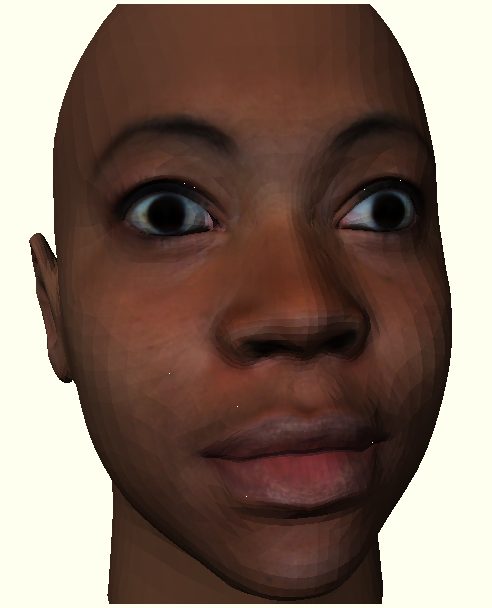
\includegraphics[width=0.7\textwidth]{holes-in-model.png}
\caption{Отверстия в модели при тесселляции}
\label{fig:holes-in-model}
\end{figure}

Тесселляция - прием, с помощью которого можно увеличить количество
многоугольников в полигональной трёхмерной модели. В процессе тесселляции
объектов, составленных целиком из треугольных полигонов \footnote{В случае
использования четырехугольных полигонов добавление новых вершин необязательно,
достаточно поделить диагональю каждый полигон пополам}, необходимо добавлять
новые вершины. В этом крылась первая проблема: объекты движка ``Three.js'',
загруженные в буферы WebGL, не могут изменить количество вершин, содержащихся в
их геометрии. Так как объект загружается в буферы WebGL при первом отображении
сцены, то для обхода этой проблемы нужно было либо тесселлировать объекты только
один раз до необходимого размера ребра непосредственно после загрузкой и до
отображения сцены, либо динамически тесселлировать объект, удалять его со сцены
и пересоздавать. Преимущество первого метода над вторым в том, что он не
затрагивает производительность приложения и несомненно является более простым в
реализации, однако он не позволяет добиться динамической тесселляции, которая
становится доступной при использовании второго метода. При разработке
планировалось опробовать алгоритм тесселляции с использованием первого метода, а
потом перейти на динамическую тесселляцию при достижении хороших результатов на
первом этапе.

При предварительном тесселлировании объектов и их дальнейшем отображении была
выявлена серия проблем.

\begin{itemize}
    \item При тесселлировании простейших геометрических фигур с четырехугольными
    гранями сбиваются цвета граней
    \item При тесселлировании загруженных *.OBJ-объектов в модели появляются
    отверстия в местах стыках граней
\end{itemize}

Если четырехугольные грани являются довольно редким объектов при задании
геометрии объектов, то второй недостаток существенен при работе с моделями.
Самостоятельное изучение кода тесселляции никаких результатов в
исправлении недостатка алгоритма не дало. Отчет об ошибке вместе с примерами
кода был отправлен разработчикам, а изменения в коде приложения,
связанные с тесселляцией, были вынужденно откачены назад.

\subsubsection{Шина событий}

В процессе разработки приложения встала проблема организации двусторонних
коммуникаций,
которые включали бы в себя как сообщения от отображения к контроллеру, так и
обратные сообщения от контроллера к отображению, инициированные моделью.
Потребность в такого рода взаимодействиях возникла в связи с необходимостью
адаптировать пользовательский интерфейс исходя из тех действий, которые делает
пользователь. Например, если включена опция автоматического вращения модели,
но пользователь попытался самостоятельно повернуть объект с помощью мышки, то
соответствующая опция должна выключиться, а галочка, сигнализирующая об активном
состоянии опции, стать неактивной.

Для решения этой проблемы было решено добавить в архитектуру глобальный объект
\texttt{EventBus}, представляющий собой шину событий.

\begin{lstlisting}
// jQuery based implementation of event bus

var EventBus = {
    subscribe: function(event, fun) {
        $(this).bind(event, fun);
    },
    publish: function(event, arg) {
        $(this).trigger(event, arg);
    }
}
\end{lstlisting}

Шина событий - объект, реализующий простой интерфейс из двух методов:
\begin{enumerate}
    \item \texttt{subscribe(event, callback)} - подписаться на событие
    \texttt{event} с помощью функции обратного вызова \texttt{callback}
    \item \texttt{publish(event, arg)} - вызвать событие
    \texttt{event} с параметром \texttt{arg}
\end{enumerate}

Реализация этого интерфейса, представленная в рамках проекта, основывается на
движке jQuery. События задаются строковыми литералами, составленными по правилу
``<Имя класса>:<имя события>''. Правило, составленное таким образом, позволяет
исключить нежелательные пересечения в именах событий. Важно отметить, что на
данный момент следование этому правилу нигде не проверяется и остается на
совести разработчика.

Благодаря шине событий модель приложения получает возможность оповещать
заинтересованных в любых своих внутренних изменениях. Таким образом контроллер
не только передает события от отображения к модели, но и, обрабатывая
соответствующие события модели, получает возможность адаптировать интерфейс так,
чтобы он соответствовал актуальному состоянию модели.

\subsubsection{Инструмент ``Деформация''}

Базовым средством изменения геометрии фигуры является инструмент ``деформация''.
С помощью этого инструмента пользователь может скорректировать геометрию
загруженного объекта.

Использование инструмента происходит по следующей схеме

\begin{enumerate}
    \item Пользователь активирует инструмент в меню инструментов
    \item После наведения мышки на модель, появляется сфера, демонстрирующая
    изменения, которые произойдут с геометрией после применения инструмента на
    этом участке модели.
    \item После одиночного щелчка мыши вершины геометрии, которые попали во
    внутрь сферы, будут спроецированы на ее переднюю поверхность
\end{enumerate}

Инструмент реализован в рамках поведенческого шаблона Strategy. Интересной
особенностью этого инструмента является то, что, ввиду необходимости добавлять
схематичную сферу на сцену для демонстрации последствий деформации, инструмент
вынужден вмешиваться в процесс отображения сцены, при этом не добавляя
дополнительных логических связей между собой и другими модулями приложения. Это
было достигнуто следующим образом.

При создании инструмента (а инструменты создаются непосредственно перед моментом
своей установки) в личном пространстве имен сохраняется функция,
выполняющую отображение сцены.

\begin{lstlisting}
function ModifyingStrategy(mobject) {
    this.managedObject = mobject;
    this.formerRender = mobject.render;
}
\end{lstlisting}

Теперь, в связки с возможностью передавать функциям любой объект,
выступающий в роли ``this'', у нас есть возможность полностью подменить функцию
отображения сцены

\begin{lstlisting}
ModifyingStrategy.prototype.setUp = function() {
    var gthis = this;
    this.managedObject.render = function() {
        // Adding sphere is needed
        ....
        // Calling original rendering method
        gthis.formerRender.call(this);
    }
}
\end{lstlisting}

В класс-ориентированных языках программирования подобный прием мог быть
реализован с помощью наследования и переопределения
виртуальных функций, с последующим вызовом супер-реализации этой функции.

Для того, чтобы задать правильные координаты сферы в сцене, необходимо решить
задачу нахождения координат точки в трехмерном пространстве сцены, на которую
указывает пользователь с помощью мышки. Задача взаимодействия
мышкой с трехмерной сценой является типовой, и в фреймворке ``Three.js'' есть
стандартное
средство для ее решения. Таким средством является объект \texttt{Ray}, который
представляет собой луч, выходящий из точки, и который может быть пересечен с
объектами сцены. Результатом пересечения будет массив точек пересечения,
каждая из которых, однако, задана в локальной координатной системе пересекаемого
объекта. Так как для создания схематичной сферы требуются координаты сцены, то
полученную точку пересечения необходимо перевести из локального пространства
объекта в пространство сцены.

К сожалению, эта задача не решена на уровне фреймворка. Поэтому для её решения
можно
воспользоваться матрицей $matrixWorld$, которая
есть у каждого объекта и которая описывает линейный оператор, переводящий точки
пространства сцены в точки пространства объекта. Благодаря тому, что оператор
является биективным, то для него однозначно определен обратный, который
определяется матрицей $matrixWorld^{-1}$. Таким образом
координаты точки пересечения в пространстве сцены могут быть получены следующим
образом

\begin{lstlisting}
var v = intersection.point.clone();
var m = new THREE.Matrix4().getInverse(mesh.matrixWorld);
m.multiplyVector3(v);
\end{lstlisting}

Теперь рассмотрим непосредственно работу самого алгоритма трансформации. После
того, как пользователь кликнул мышью на какой-либо участок геометрии, все точки,
попавшие внутрь сферы, проецируются на переднюю поверхность сферы. Определим
работу алгоритма более конкретно

А алгоритма есть два параметра: радиус сферы трансформации $R$, а так же
коэффициент заглубления $K$. Их назначение будет пояснено ниже

\begin{enumerate}
    \item Определим точку $p$ модели, на которую кликнул пользователь.
    \item Определим внешнюю нормированную нормаль $\vec{n}$ к модели в этой
    точке. Внешняя нормаль определяет направление проецирования точек геометрии
    \item Рассмотрим вектор $\vec{v} = - R \cdot \vec{n}$,
    направленный в противоположную сторону относительно вектора деформации и по
    модулю равный $R$. Центр сферы $S$ принимается равным $с = p + K \cdot \vec{v}$
    а за радиус берется $R$
    \item Для каждой вершины $u$ геометрии, попадающей внутрь сферы $S$, проверим,
    лежит ли она в первой половине сферы. Для этого достаточно посчитать
    скалярное произведение радиус-векторов
    $$(\vec{u}-\vec{c}) \cdot \vec{n} = |\vec{u}-\vec{c}| \cdot |\vec{n}| \cdot
    cos(\vec{u} \wedge \vec{n})$$
    Знак скалярного произведения будет меньше нуля в том случае,
    если точка лежит во второй половине сферы, удаленной от зрителя. В таком
    случае эту точку проецировать не надо.
    \item Для каждой точки, подлежащей трансформации, происходит проецирование на
    поверхность сферы по направлению, заданному вектором деформации $\vec{n}$
\end{enumerate}

Операция проецирования эквивалентна решению следующей задачи.

Рассмотрим прямую, заданную радиус-вектором $\vec{s}$, задающим точку, которую
надо спроецировать, и вектором направления проекции $\vec{d}$. Тогда точки этой
прямой выражаются следующим уравнением
$$ \vec{p}_{line} = \vec{s} + k \cdot \vec{d} $$

В свою очередь, точки сферы с центром в $(x_c, y_c, z_c)$ в общем виде задаются
следующим уравнением
$$ (x-x_c)^2 + (y-y_c)^2 + (z-z_c)^2 = R^2 $$

Подставив первое уравнение во второе, мы найдем один или два корня. В случае
нахождения одного корня точка уже является спроецированной на сферу.

В случае нахождения двух корней $k_1, k_2$ мы получаем две точки пересечения
сферы и прямой, и при этом если изначальная точка $\vec{s}$ находилась внутри
сферы, то корни будут разных знаков. Так как нас интересует проекция на переднюю
половину сферы, то проекцией будет точка, полученная положительным корнем.

\subsubsection{Использование технологии AJAX}

В ходе разработки сервиса было установлено, что пользователь в процессе работы
совершает многочисленные запросы к серверу, как для загрузки модели в окно
редактора, так и для добавления новой obj-модели в инспектор объектов и вызова
серверных вычислений. Каждое действие требовало перезагрузки страницы, что
значительно ухудшало опыт использования приложения.

В связи с этими причинами было решено полностью перейти к взаимодействию между
клиент-серверной частью по средствам технологии AJAX (Asynchronous Javascript
And XML). Технология AJAX базируется на двух основных принципах

\begin{enumerate}
    \item Использование технологии обращения к серверу без перезагрузки страницы
    \item Использование \texttt{DHTML} для динамического изменения содержимого
    страницы
\end{enumerate}

Классические примеры применения технологии AJAX используют JavaScript-объект
XMLHttpRequest. Однако этот подход чреват проблемами совместимости с некоторыми
старыми браузерами. Например, в браузере Microsoft Internet Explorer объект
XMLHttpRequest не определен, однако есть его аналог с другим именем. Поэтому для
его создания рекомендуется применять подобный код

\begin{lstlisting}
function getXmlHttp(){
  var xmlhttp;
  try {
    xmlhttp = new ActiveXObject("Msxml2.XMLHTTP");
  } catch (e) {
    try {
      xmlhttp = new ActiveXObject("Microsoft.XMLHTTP");
    } catch (E) {
      xmlhttp = false;
    }
  }
  if (!xmlhttp && typeof XMLHttpRequest!='undefined') {
    xmlhttp = new XMLHttpRequest();
  }
  return xmlhttp;
}
\end{lstlisting}

Изучение тематических ресурсов, посвященных этой технологии, показало, что
объекты XMLHttpRequest, полученные универсальным способом, описанным выше,
несколько отличаются по функциональности. В качестве примера можно привести
метод \texttt{abort()}, который должен обрывать текущий запрос, однако в случае
Internet Explorer этого не делает.

Таким образом, использование XMLHttpRequest порождает целую серию проблем не
только по написанию кросс-браузерного кода, но и по его дальнейшему
сопровождению. Для их решения было решено использовать фреймворк
\texttt{jQuery}, который по мимо специальных функций, ``оборачивающих''
XMLHttpRequest и решающий таким образом многочисленные проблемы с его
использованием, предоставляет поддержку языка запросов к элементам страницы
``XPath'', что значительно облегчает динамическое манипулирование содержимым
страницы.

\subsection{Серверные технологии}

\subsubsection{Фреймворк ``Express.js''}

При разработке web-сервиса были поставлены следующие общие задачи:

\begin{enumerate}
    \item Требуется некоторый механизм сопоставления действий адресам, запрошенным
    пользователем
    \item Необходимо поддерживать возможность генерации html-страниц на основе
    информации, доступной серверу в момент запроса
\end{enumerate}

Для решения этих задач было решено использовать фреймворк для разработки
REST-сервисов на платформе ``Node.js'' под названием ``Express.js''. Фреймворк
состоит из нескольких частей и решает следующие задачи:

\begin{enumerate}
    \item маршрутизация запросов пользователя
    \item разбор тела запроса (в случае передачи форм и загрузки файла)
    \item рендеринг представлений\footnote{подразумевается генерация HTML-кода
    web-страниц, который будет отправлен в ответ на запрос
    пользователя} на основе набора параметров
\end{enumerate}

Фреймворк позволяет строить таблицу маршрутизации запросов с помощью
обработчиков основных глаголов REST-сервисов: REST, POST, PUT, DELETE. Тут
необходимо особо отметить, что протокол связи HTTP 1.0 поддерживает только три
метода: HEAD, GET, POST, а язык разметки HTML вплоть до версии 4.0 не содержит
методов PUT и DELETE в качестве опций для отправки форм на сервер.

Поэтому для того, чтобы ``Express.js'' мог осуществлять маршрутизацию запросов по
отправке форм с глаголами PUT и DELETE, формы должны содержать дополнительно
скрытое поле с именем \texttt{method} и значением, содержащим имя желаемого
метода.

\subsubsection{Рендеринг web-страниц}

Основной задачей рендеринга является формирование страницы, содержащей
информацию, специфическую для данного запроса. Наиболее естественным подходом
для создания таких страниц является использование всевозможных
HTML-препроцессоров, которым можно передать дополнительные параметры.
Так, например, на платформе ``Ruby on Rails'' рендеринг представлений
осуществляется
за счет обработки \texttt{erb}-файлов \footnote{embedded ruby file}, а на
платформе ``Java EE'' для этих целей используются Java Server Pages. Стандартом
де-факто для фреймворка ``Express.js'' является технология Jade.

Jade --- препроцессор HTML-кода, написанный на языке JavaScript. Jade
преобразует код, написанный на специально разработанном DSL\footnote{Domain
Specific Language} (далее - просто язык Jade), в HTML-разметку. Одним из
несомненных достоинств языка Jade является двумерный синтаксис, хорошо себя
зарекомендовавший для описания структур с глубокой вложенностью, а потому
хорошо подходящим для описания компонентов и элементов HTML страницы.

Показательным примером использования технологии Jade будет следующий листинг.
Рассмотрим следующий код на языке Jade

\begin{lstlisting}
!!!
html(lang="en")
  head
    title= pageTitle
    script(type='text/javascript')
      if (foo) {
         bar()
      }
  body
    h1 Jade - node template engine
    #container
      if youAreUsingJade
        p You are amazing
      else
        p Get on it!
\end{lstlisting}

Препроцессор, запущенный на данном коде с параметром \texttt{pageTitle = "Hello,
Jade"}, генерирует следующих HTML-код

\begin{lstlisting}[language=html]
<!DOCTYPE html>
<html lang="en">
  <head>
    <title>Jade</title>
    <script type="text/javascript">
      if (foo) {
        bar()
      }
    </script>
  </head>
  <body>
    <h1>Jade - node template engine</h1>
    <div id="container">
      <p>You are amazing</p>
    </div>
  </body>
</html>
\end{lstlisting}

Этот пример иллюстрирует основной способ передачи параметров и использования в
тексте шаблона.

\subsubsection{Загрузка *.obj-объектов}

Одной из главных возможностей приложения является динамическая загрузка
трехмерных объектов, заданных в открытом формате OBJ. К сожалению, сорок восьмая
ревизия фреймворка ``Three.js'', которая используется в приложении, не позволяет
осуществлять динамическую загрузку непосредственно OBJ-моделей и требует
предварительной
конвертации файлов в специального вида JSON-объекты. В стандартную поставку
библиотеки входит скрипт \texttt{convert\_obj\_three.py}, написанный на языке
Python, созданный специально для этих целей. К сожалению, язык
скрипта не позволяет запустить его в браузере на стороне пользователя, а объем
кода в 48 килобайт делают задачу портирования достаточно трудоемкой чреватой на
многочисленные ошибки.

В качестве решения было решено ввести в интерфейс приложения инспектор объектов,
который бы отображал список уже загруженных и объектов,
доступных для динамической загрузки в редактор. Пользователь имеет возможность
удалить любой из объектов инспектора, а так же добавить новые объекты с помощью
специальной формы. При добавления нового объекта пользователем происходит
следующая цепочка событий

\begin{enumerate}
    \item Пользователь через специальную форму выбирает расположенные локально
    на его компьютере OBJ-объекты, которые он хочет увидеть в браузере
    \item Выбранные файлы загружаются на сервер, где с помощью скрипта из
    пакета поставки фреймворка ``Three.js'' преобразуются в необходимый формат и
    сохраняются
    \item При получении успешного ответа сервера при загрузке файлов клиент
    автоматически отправляет запрос на получение нового списка объектов для
    отображения в инспекторе объектов. Пользователь может загрузить любой
    объект из списка
\end{enumerate}

Ввиду того, что типичный сценарий использования приложения не подразумевает
наличия большого количества преобразованных объектов одновременно, было решено
организовать их хранилище на основе файловой системы (ФС). Таким образом все
преобразованные объекты хранятся на сервере в специальной папке
\texttt{./objects}, а основные операции были организованы следующим
образом

\begin{itemize}
    \item ADD. Эта команда должна добавить новый объект в хранилище. В
    случае ФС создается новая папка с именем таким же, как имя объекта, и все
    файлы, относящиеся к объекту, сохраняются в ней
    \item LIST. Эта команда должна вернуть список имен всех объектов. В
    случае ФС она возвращает список имен директорий, находящихся в папке
    \texttt{./objects}
    \item REMOVE. Эта команда должна удалить объект по его имени. В случае
    ФС она удаляет папку с соответствующим именем.
\end{itemize}

Для вызовов внешних процедур изнутри ``Node.js'' использовался метод exec модуля
``child\_process''. Для каждого из действий, вовлекающих использование внешних
вызовов, была разработана соответствующая оболочка на языке JavaScript.

\subsection{Серверные вычисления}

\subsubsection{Формулировка задачи}

Кроме необходимости поддерживать унаследованный от ранее разработанный
desktop-приложений код, было установлено, что возможности скриптового языка
JavaScript в проведении сложных вычислений не велики. Таким образом встала
задача использования вычислительно сложных алгоритмов для работы с трехмерной
геометрией при условии невозможности реализации этих алгоритмов на языке
JavaScript для исполнения на стороне клиента.

Для решения этой проблемы было решено использовать удаленные серверные
вычисления. При таком подходе необходимо ввести в архитектуру приложения еще
одну сущность - сервер высокопроизводительных вычислений (СВВ). Для начала
опишем роль, которую играет этот объект при выполнении серверных вычислений.

При таком подходе для обсчета геометрии с помощью какого-либо алгоритма будут
сделаны следующие шаги.

\begin{enumerate}
    \item Данные о текущем состоянии геометрии фигуры, отображенной в браузере,
    считываются и передаются на сервер
    \item Сервер сериализует эти данные и передает с помощью какого-либо
    транспорта в СВВ
    \item СВВ десериализует эти данные и передает их на вход алгоритму
    \item СВВ получает результат работы алгоритма, сериализует их и с
    помощью того же транспорта передает на сервер
    \item Сервер десериализует данные и отправляет их клиенту
\end{enumerate}

Таким образом структурно СВВ является некоторой оболочкой над алгоритмом (или
группой алгоритмов), осуществляющий операции сериализации и десериализации
данных, а так же передачи их по назначению с помощью какого-либо транспортного
уровня.

Важно отметить, что данная технология подразумевает наличие модуля сериализации
и десериализации данных как на стороне сервера, так и на стороне СВВ, причем
эти модули должны оперировать одним и тем же форматом данных, но быть
написанными на разных языках программирования (в нашем случае, с одной стороны -
на JavaScript, с другой стороны на С++).

Задача реализации СВВ, а так же модуля сериализации и десериализации данных на
JavaScript была решена с помощью автоматической генерации кода по заданной
модели и использованием технологии Apache Thrift.

\subsubsection{Применение thrift-технологии}

Apache Thrift - технология, разработанная для создания приложений на
разных языках программирования. Для организации такого взаимодействия между
компонентами, написанными на двух языках, требуется использовать модули
сериализации и десериализации, а так же модуль, ответственный за транспортный
уровень передачи
данных, для каждого из языков, участвующих во взаимодействии. Такие модули
создаются процессом генерации кода, который происходит на основе описанной на
специальном языке Thrift модели.

Thrift модель позволяет описывать две сущности: данные, которыми обмениваются
стороны взаимодействия, и сигнатуры процедур, которые одна сторона
предоставляет для удаленного вызова. Одна из сторон взаимодействия является
клиентской и инициирует взаимодействие путем вызова процедур, предоставленных
серверной стороной. Таким образом на основании этих данных Apache Thrift
генерирует код описания данных, код, выполняющий сериализацию и десериализацию
данных, а так же их отправку и прием с помощью транспортного уровня. Кроме этого
генератор создает файл ``MainService\_server.skeleton.cpp'', создержащий наброски
серверной части взаимодействия с заглушками вместо процедур удаленного вызова.

\begin{lstlisting}[caption={Пример описания модели и сервиса для технологии
Thrift}]
struct Point {
    1: double x,
    2: double y
}

service ScaleService {
    Point scalePoint(1:Point point, 2:int scalar)
}
\end{lstlisting}

В нашем случае в качестве сервисов выступают конкретные алгоритмы, выполняющие
удаленные вычисления. Так как эти алгоритмы могут добавляться и исчезать в
процессе развития проекта, то необходимо изменять соответствующим образом
описание сервиса в файле описания thrift, а затем перегенерировать все файлы
ввиду внесенных изменений. После генерации файлов необходимо будет обновить
файл ``server.cpp'', добавив соответствующие директивы ``include'' и исправив
заглушки на вызов соответствующих алгоритмов.

Из всего вышесказанного следует, что для того, чтобы добавить новый алгоритм в
систему, потребуется знание
формата файлов Thrift, а так же четкое понимание внутренней структуры сервиса,
что значительно усложняет процесс расширения функционала всего приложения.

Для того, чтобы облегчить процесс добавления новых алгоритмов, был написан
скрипт ``generate.sh'' для оболочки ``bash'', занимающийся автоматизацией этих
операций. При использовании этого скрипта, процесс добавления новых алгоритмов
для обработки геометрии сводится к следующей цепочки действий
\begin{enumerate}
    \item Файл реализации \texttt{*.cpp} и файл заголовка \texttt{*.h}
    помещаются в папку \texttt{./thrift/algo}. Файл заголовка должен содержать
    только описания функций, обрабатывающих геометрию объекта.
    \item Запускается команда ``bash generate.sh'' из папки \texttt{./thrift},
    которая компилирует серверную часть Thrift
\end{enumerate}

После этого сервер ``./thrift/server'' готов к использованию и может быть
запущен для предоставления сервиса по удаленному использованию процедур. Кроме
этого, на стороне серверной части приложения ``Node.js'' список функций,
доступных для удаленного вызова, автоматически обновился.

Скрипт ``generate.sh'' совершает следующие действия
\begin{enumerate}
    \item Удаляет директории \texttt{gen-nodejs} и \texttt{gen-cpp}, очищая
    таким образом данные, полученные при предыдущих запусках скрипта.
    \item Сканирует папку, содержащую все алгоритмы пользователя, и, анализируя
    все ``*.h'' файлы, найденные в ней, создает соответствующий файл описания
    сервиса для технологии Thrift
    \item С помощью технологии Thrift и на основе файла описания сервиса и
    данных, генерирует код на языке JavaScript для платформы ``Node.js''
    \item Создает файл ``remoteComputing.js'', содержащий функции,
    соответствующие именам найденных функций пользователя. Таким образом на
    стороне серверной части вызов этих функций ничем не будет отличаться
    от вызова любой другой функции из фреймворка ``Node.js''
    \item С помощью технологии Thrift и на основе файла описания сервиса и
    данных, генерирует код на языке C++.
    \item Исправляет файл ``server.cpp'', сгенерированный технологией Thrift,
    убирая в нем заглушки и заменяя их соответствующим вызовом функций
    пользователя
    \item Исправляет использующийся транспорт сервера на соответствующий
    транспорт, используемый в js-части приложения
    \item Компилирует файл ``server.cpp'', получая готовое серверное приложение.
\end{enumerate}

Стоит отдельно отметить пункт 2, включающий в себя анализ ``*.h'' файлов
пользователя. Для этой цели было решено использовать утилиту ``ctags''.
Благодаря ей список функций, определенных среди всех файлов с алгоритмами, можно
получить следующим образом
\begin{lstlisting}[language=bash]
    ctags -x --c-kinds=p *.h | cut -f1 -d' '
\end{lstlisting}

\subsubsection{Десериализация вещественного типа в Node-Thrift}

В процессе интеграции технологии Apache Thrift в приложение был использован
достаточно молодой модуль ``Node-Thrift'' для платформы ``Node.js'', включающий
в себя
необходимый код для передачи данных с помощью транспорта, а так же сериализацию
и десериализацию простейших типов данных.

К сожалению, после первых экспериментов было установлено, что модуль работает
некорректно. В качестве подтверждения был написан следующий echo-сервис, который
работал ошибочно в условиях взаимодействия компонентов на языках ``Node.js'' и
C++.

\begin{lstlisting}
service EchoService {
    double echo(1:double msg);
}
\end{lstlisting}

В результате генерации кода на основании этого файла описания данных,
клиентское приложение всегда получало 0 в качестве ответа на удаленный
вызов процедуры. Однако проблемы не возникало при использовании любых других
типов данных, отличных от double. Кроме того, проблемы не возникало при
использовании языка Ruby для генерации клиентской части. Из этого следовало, что
ошибка кроется в библиотеке ``Node-Thrift'' для платформы ``Node.js''.
Соответствующий отчет об ошибке был отправлен разработчику.

Ввиду необходимости продолжать разработку, была предпринята попытка устранить
ошибку в библиотеке Node-Thrift самостоятельно. После изучения исходных
кодов модуля было установлена, что ошибка возникает на этапе десериализации
данных и связана с неправильным декодированием 8-байтного вещественного типа.
После обнаружения неисправность была устранена, а соответствующий патч,
исправляющий проблему, был выслан разработчику модуля.

\section{Тестирование}

Для того, чтобы установить перспективы использования разработанного web-сервиса,
была проведена серия экспериментов. Эксперименты замеряли одну из следующих
величин:
\begin{enumerate}
    \item FPS (Frames per second) - количество итераций отображения
    трехмерной сцены в секунду. Считается, что значения в 30FPS и более являются
    достаточно комфортными для человеческого восприятия.
    \item Время отклика сервера при использовании серверных
    вычислений. Вычисляется как временной промежуток между обновленным
    результатом на клиенте по выполнению серверных вычислений и непосредственной
    инициацией процесса на клиенте.
\end{enumerate}

Каждый эксперимент имел целью исследование зависимостей между количеством
полигонов в модели и тем или иным изучаемым параметром. Исследования проводились
на четырех различных моделях

\begin{center}
\scalebox{0.8}{%
    \begin{tabular}{ | c | c | c | c | c | c | }
    \hline
     Имя модели & \textbf{couch1} & \textbf{Jane\_solid\_obj} & \textbf{ladybird} & \textbf{Woman-head} & \textbf{Mini-cooper} \\ \hline
     Количество полигонов & 3098 & 12334 & 23496 & 114344 & 254714  \\
    \hline
    \end{tabular}
}
\end{center}

Эксперименты проводились на тестовом стенде следующей конфигурации:
\begin{itemize}
    \item Браузер: Google Chrome v.19.0
    \item Процессор: Intel Core i5, 1.7ГГц, кэш-память третьего уровня в 3 Мб
    \item Память: 4 ГБ DDR3 1333МГц
    \item Графический процессор: Intel HD Graphics 3000 с памятью 384
\end{itemize}

\subsection{Тест: просмотр модели}

Эксперимент проводился с целью определения возможностей статического
рендеринга трехмерных моделей средствами технологии WebGL и фреймворка
``Three.js''. В рамках исследования был проведен ряд тестов, каждый из которых
состоит из следующей последовательности шагов:
\begin{enumerate}
    \item В web-приложение загружается трехмерная модель
    \item С загруженной моделью совершают ряд операций поворота
    и масштабирования
    \item Результатом теста является среднее значение FPS, полученное
    за время работы с моделью
\end{enumerate}

\subsubsection{результаты}
\begin{center}
\scalebox{0.7}{%
    \begin{tabular}{ | c | c | c | c | c | c | }
    \hline
    Количество полигонов & 3098 & 12334 & 23496 & 114344 & 254714 \\
    \hline
    FPS & 60 & 60 & 60 & 60 & 59 \\
    \hline
    \end{tabular}
}
\end{center}

\subsubsection{выводы}

Из результатов эксперимента видно, что технология WebGL вместе с фреймворком
``Three.js'' отлично справляется с рендерингом трехмерных моделей.

\subsubsection{Тест: локальное изменение модели}

Эксперимент проводился с целью определения возможностей динамического
изменения трехмерных моделей на стороне клиента. Каждый из тестов, проведенный в
рамках исследований, состоит из следующей последовательности шагов:

\begin{enumerate}
    \item В web-приложение загружается трехмерная модель
    \item С загруженной моделью с помощью инструмента для локального изменения
    геометрии совершается ряд преобразований
    \item Результатом теста является среднее значение FPS, полученное за время
    работы с моделью
\end{enumerate}

\subsubsection{результаты}
\begin{center}
\scalebox{0.8}{%
    \begin{tabular}{ | c | c | c | c | c | c | }
    \hline
    Количество полигонов & 3098 & 12334 & 23496 & 114344 & 254714 \\
    \hline
    FPS & 60 & 41 & 22 & 6 & 2 \\
    \hline
    \end{tabular}
}
\end{center}

\subsubsection{выводы}

Эксперимент показала явную регрессию производительности при увеличении
количества полигонов в модели. Это связано в первую очередь с тем, что
инструмент локального изменения геометрии добавляет в процесс рендеринга
дополнительную операцию пересечения луча со сценой (операция необходима для
того, чтобы расположить схематичную сферу трансформации на модели).

Операция пересечения луча с объектом, в свою очередь, написана на языке
JavaScript и работает за $O(N)$, где $N$ - количество полигонов в объекте.
Именно такую зависимость FPS от количества полигонов можно наблюдать в
результате эксперимента.

Эксперимент демонстрирует неприменимость текущей реализации для
высоко-полигональных моделей. Можно перечислить следующие пути для решения этой
проблемы, которые могут быть реализованы в дальнейшем
\begin{enumerate}
    \item Путем изменения схемы взаимодействия пользователя с объектом можно
    исключить необходимость в отрисовке схематичной сферы деформации
    \item Заметим, что за единицу времени сфера трансформации может сдвинуться
    на не очень большое расстояние. Такой подход дает возможность для попыток
    реализации множественных инкрементальных алгоритмов, которые делают
    первоначальное размещение сферы за время $O(N)$, однако после этого
    незначительные изменения в положении сферы могут быть пересчитаны за гораздо
    меньшее количество операций.
\end{enumerate}

\subsubsection{Тест: серверные вычисления}

Эксперимент проводился с целью определения эффективности технологии серверных
вычислений.

\subsubsection{результаты}
\begin{center}
\scalebox{0.9}{%
    \begin{tabular}{ | c | c | c | c | c | c | }
    \hline
    Количество полигонов & 3098 & 12334 & 23496 & 114344 & 254714 \\
    \hline
    Задержка, мс & 231 & 709 & 2682 & 7715 & 36996 \\
    \hline
    \end{tabular}
}
\end{center}

\subsubsection{выводы}

При анализе результатов эксперимента оказалось, что большая часть потраченного
времени уходила на процессы сериализации и передачи данных в модуле
``Node-Thrift''. Данная проблема уже замечена и решается разработчиком модуля,
что дает надежду на скорое ее разрешение в ближайшем будущем.

\section{Результат}

Результатом дипломной работы стал web-сервис для работы с трехмерными объектами.
Сервис предоставляет функционал по обработке трехмерных объектов, а именно:
\begin{itemize}
    \item Загрузку трехмерных моделей в формате *.OBJ
    \item Просмотр трехмерных моделей с функциями поворота, масштабирования
    и режимом автоматического вращения
    \item Локальное изменение трехмерных моделей с помощью специального инструмента
    \item Изменение трехмерных моделей за счет алгоритмов,
    реализованных на стороне сервера на языке С++
\end{itemize}

Разработанный сервис предоставляет следующие возможности модульного
расширения:
\begin{enumerate}
    \item Возможность добавления инструментов для взаимодействия с
    трехмерным объектом
    \item Возможность добавления алгоритмов на языке С++ для серверной обработки
    геометрии
\end{enumerate}

\begin{figure}[htb]
\centering
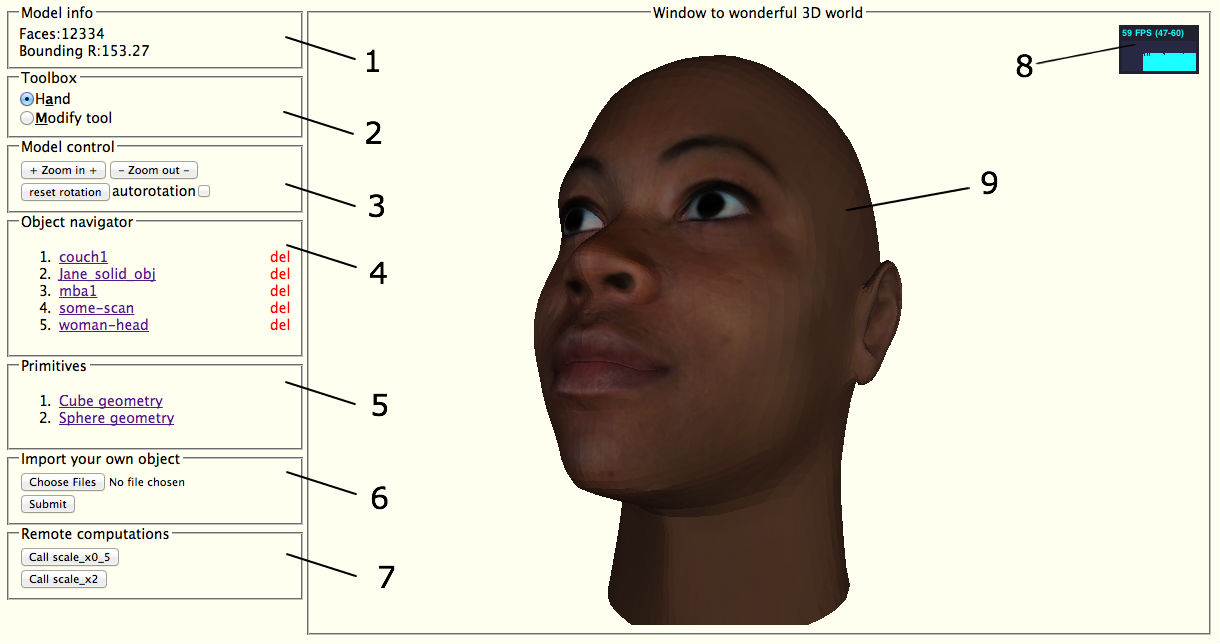
\includegraphics[width=1.0\textwidth]{ui.jpg}
\caption{Интерфейс приложения}
\label{fig:ui}
\end{figure}

Элементы интерфейса
\begin{description}
    \item[1 Информация] Здесь предоставляется информация о количестве
    полигонов и радиусе описанной окружности модели.
    \item[2 Инструменты] Набор инструментов для
    взаимодействия с моделью. Для выбора возможно использование быстрых клавиш
    \item[3 Управление моделью] Управление объектом: приближение, удаление,
    автоматическое вращение объекта
    \item[4 Инспектор объектов] База преобразованных OBJ-файлов, доступных для
    динамической загрузки в редактор. Нажатие ссылки ``del'' рядом с каждым объектом
    приведет к его удалению из базы.
    \item[5 Графические примитивы] Загрузка графических примитивов в поле
    редактора
    \item[6 Импорт OBJ-объектов] Форма для добавления OBJ-объектов в инспектор
    объектов.
    \item[7 Серверные вычисления] Список доступных функций преобразования
    геометрии, заданных и выполняемых на стороне сервера
    \item[8 FPS гистограмма] Статистика по количеству FPS
    \item[9 3D сцена] Сцена с трехмерным объектом
\end{description}


\end{document}
